% JW-FD Universe (MDPI) Article manuscript
\documentclass[universe,article,submit,pdftex,moreauthors]{Definitions/mdpi}

\usepackage{amsmath}
\usepackage{booktabs}
\usepackage{tikz}
\usepackage{pgfplots}
\pgfplotsset{compat=1.18}
\usetikzlibrary{positioning,arrows.meta,shapes.geometric}

\firstpage{1}
\makeatletter
\setcounter{page}{\@firstpage}
\makeatother
\pubvolume{1}
\issuenum{1}
\articlenumber{0}
\pubyear{2026}
\copyrightyear{2026}
\datereceived{ }
\daterevised{ }
\dateaccepted{ }
\datepublished{ }

\Title{JW-FD: A Long Horizon Multimodal Solar Flare Forecasting Dataset for Large Language Models}

\newcommand{\orcidauthorA}{0009-0003-1447-2439}

\Author{Shao Mingfu $^{1}$\orcidA{}, Lin Jiaben $^{1,}$*, Wang Hui $^{1}$, Tong Liyue $^{1}$, Yang Chen $^{1}$, Zhang Yin $^{1}$ and Li Yuyang $^{1}$}

\AuthorNames{Shao Mingfu, Lin Jiaben, Wang Hui, Tong Liyue, Yang Chen, Zhang Yin, and Li Yuyang}

\address{%
$^{1}$ \quad National Astronomical Observatories, Chinese Academy of Sciences, Beijing 100101, China; jiabenlin@bao.ac.cn}

\corres{Correspondence: jiabenlin@bao.ac.cn}

\abstract{Solar flares drive severe space weather hazards, and forecasting flare occurrence from photospheric magnetograms remains a central challenge for heliophysics and operational forecasting services. Machine learning and multimodal large language model methods require long horizon datasets in which images, magnetic features, and flare labels are coregistered in space and time. We present \textbf{JW-FD} (JW-Flare Dataset), a 15 year multimodal release spanning 1~January~2011 through 31~December~2025, constructed from SDO/HMI line of sight magnetograms, NOAA Solar Region Summary reports, and NOAA X-ray flare event lists. The dataset comprises 3{,}064 independent active regions, 1{,}991{,}247 magnetograms, and 3{,}064 per region evolution videos. Each sample corresponds to 29 magnetic features, 35 flare labels, and 2 metadata columns (66~dimensions in total). Labels follow strict forecasting semantics before eruption over seven forecast horizons and four GOES intensity thresholds. An 8:1:1 split at the active region level is adopted to prevent temporal leakage between partitions. PNG branches are released at six magnetic saturation thresholds, and internal Transformer experiments on $\geq$C1.0 forecasting suggest $B_{\mathrm{th}}=1000$~G as a preliminary default, although the optimal saturation is model and task dependent. The open source construction pipeline is available at \url{https://github.com/Xiaoxuan-1/JW-FD}.}

\keyword{solar flare forecasting; magnetograms; multimodal dataset; machine learning}

\begin{document}

\section{Introduction}
\label{sec:intro}

Solar flares are among the most energetic manifestations of solar magnetic activity. Major flares (M/X class) can disrupt satellite operations, aviation communications, and power grid infrastructure. Forecasting flare occurrence before eruption from photospheric magnetograms is therefore a priority for fundamental solar physics~\cite{Shao2025review,Toriumi2019,Leka2019}.

Photospheric line of sight (LoS) magnetograms encode signatures of magnetic complexity (gradient concentrations, neutral line topology, and flux imbalance) that precede many eruptive events~\cite{Boucheron2015,Bobra2014}. Quantitative features derived from magnetograms have long supported statistical and machine learning (ML) flare forecasting models, and recent work extends this paradigm to convolutional neural networks (CNNs), vision transformers, and multimodal large language models (MLLMs) that consume both images and structured physical parameters~\cite{Shao2025jwflare}. Such methods require datasets in which visual, physical parameters, and label modalities are coregistered in space and time, together with a train/validation/test splitting scheme that prevents temporal information leakage between partitions.

Several public datasets now support data driven flare forecasting, but their coverage remains limited for long horizon multimodal modeling. Boucheron et al.\ released an active region (AR) LoS magnetogram image dataset covering 2010--2018~\cite{Boucheron2023}. Relative to Cycles~24--25, its temporal span is shorter, and it does not yet provide coregistered images, magnetic features, and configurable labels across forecast horizons and intensity thresholds.

Space-weather Helioseismic and Magnetic Imager (HMI) Active Region Patches (SHARPs) supply vector field cutouts and summary keywords that underpin many forecasting studies~\cite{Bobra2014sharp,Bobra2014}. Building on this product, Angryk et al.\ released SWAN-SF, a multivariate time series dataset of SHARP parameters covering 2010--2018~\cite{Angryk2020}, while Nishizuka et al.\ assembled and released feature databases associated with Deep Flare Net (DeFN)~\cite{Nishizuka2017,Nishizuka2018}. Subsequent work continues to organize SHARP parameter sets for operational forecasting~\cite{Abduallah2023,Florios2018}. These resources are strong for tabular and time series learning, but they do not yet jointly release magnetogram imagery, extracted features, and evolution videos for active regions under a single indexing scheme spanning Cycles~24--25.

Complementary studies assemble magnetogram or multiwavelength working datasets for CNNs, long short term memory (LSTM) networks, and related models~\cite{Huang2018,Li2020,Sun2022,Jonas2018}. As noted in recent surveys, however, many forecasting studies still rely on assemblies specific to each study that are not redistributed as a reusable long horizon multimodal dataset, which limits comparison across studies and reproducibility~\cite{Shao2025review,Bloomfield2012,Barnes2016}. More recently, SuryaBench provides a large multitask heliophysics benchmark for foundation model research, with solar flare forecasting as one of several applications~\cite{Roy2026}. Although valuable as a broad evaluation suite, it is not a dedicated multimodal flare forecasting release centered on active regions, with configurable labels across forecast horizons and a training, validation, and test split at the active region level designed to prevent temporal leakage~\cite{Leka2019}.

Taken together, these efforts leave open the need for a single long horizon multimodal dataset at the active region level that coregisters images, magnetic features, flare labels, and evolution videos under partitions that avoid temporal leakage.

\textbf{JW-FD} (JW-Flare Dataset) is designed to meet this need. It provides a single long horizon benchmark for vision models, ML, and multimodal architectures. This paper presents the dataset, its design rationale, construction pipeline, and recommended usage.
Our principal contributions are:
\begin{enumerate}
\item A \textbf{15 year multimodal release} (2011--2025) covering solar Cycles~24--25 with 1.99~million active region snapshots, supporting studies of cycle dependent flare statistics and rare X class events.
\item \textbf{Coregistered images, magnetic features, flare labels, and evolution videos}, with 66 dimensional records that link 29 magnetic features to configurable labels defined before eruption.
\item \textbf{Configurable labels} with strict forecasting semantics before eruption over seven forecast horizons and four Geostationary Operational Environmental Satellite (GOES) intensity thresholds.
\item An \textbf{8:1:1 training, validation, and test split at the active region level} that keeps all timestamps of one AR in a single partition, reducing temporal leakage for classical ML, deep vision models, and MLLMs.
\end{enumerate}

\section{Materials and Methods}
\label{sec:methods}

JW-FD is constructed with a six step automated pipeline that ingests Solar Region Summary (SRS) reports and NOAA Events X-ray (XRA) flare lists from the National Oceanic and Atmospheric Administration/Space Weather Prediction Center (NOAA/SWPC), together with Solar Dynamics Observatory (SDO)/HMI~\cite{Scherrer2012,Pesnell2012} full disk LoS magnetograms. The pipeline exports Flexible Image Transport System (FITS) crops, Portable Network Graphics (PNG) images, comma separated values (CSV) tables, and MPEG-4 (MP4) videos. Figure~\ref{fig:pipeline} summarizes the workflow; Table~\ref{tab:pipeline} lists the inputs and outputs of each step.

\begin{figure}[H]
\centering
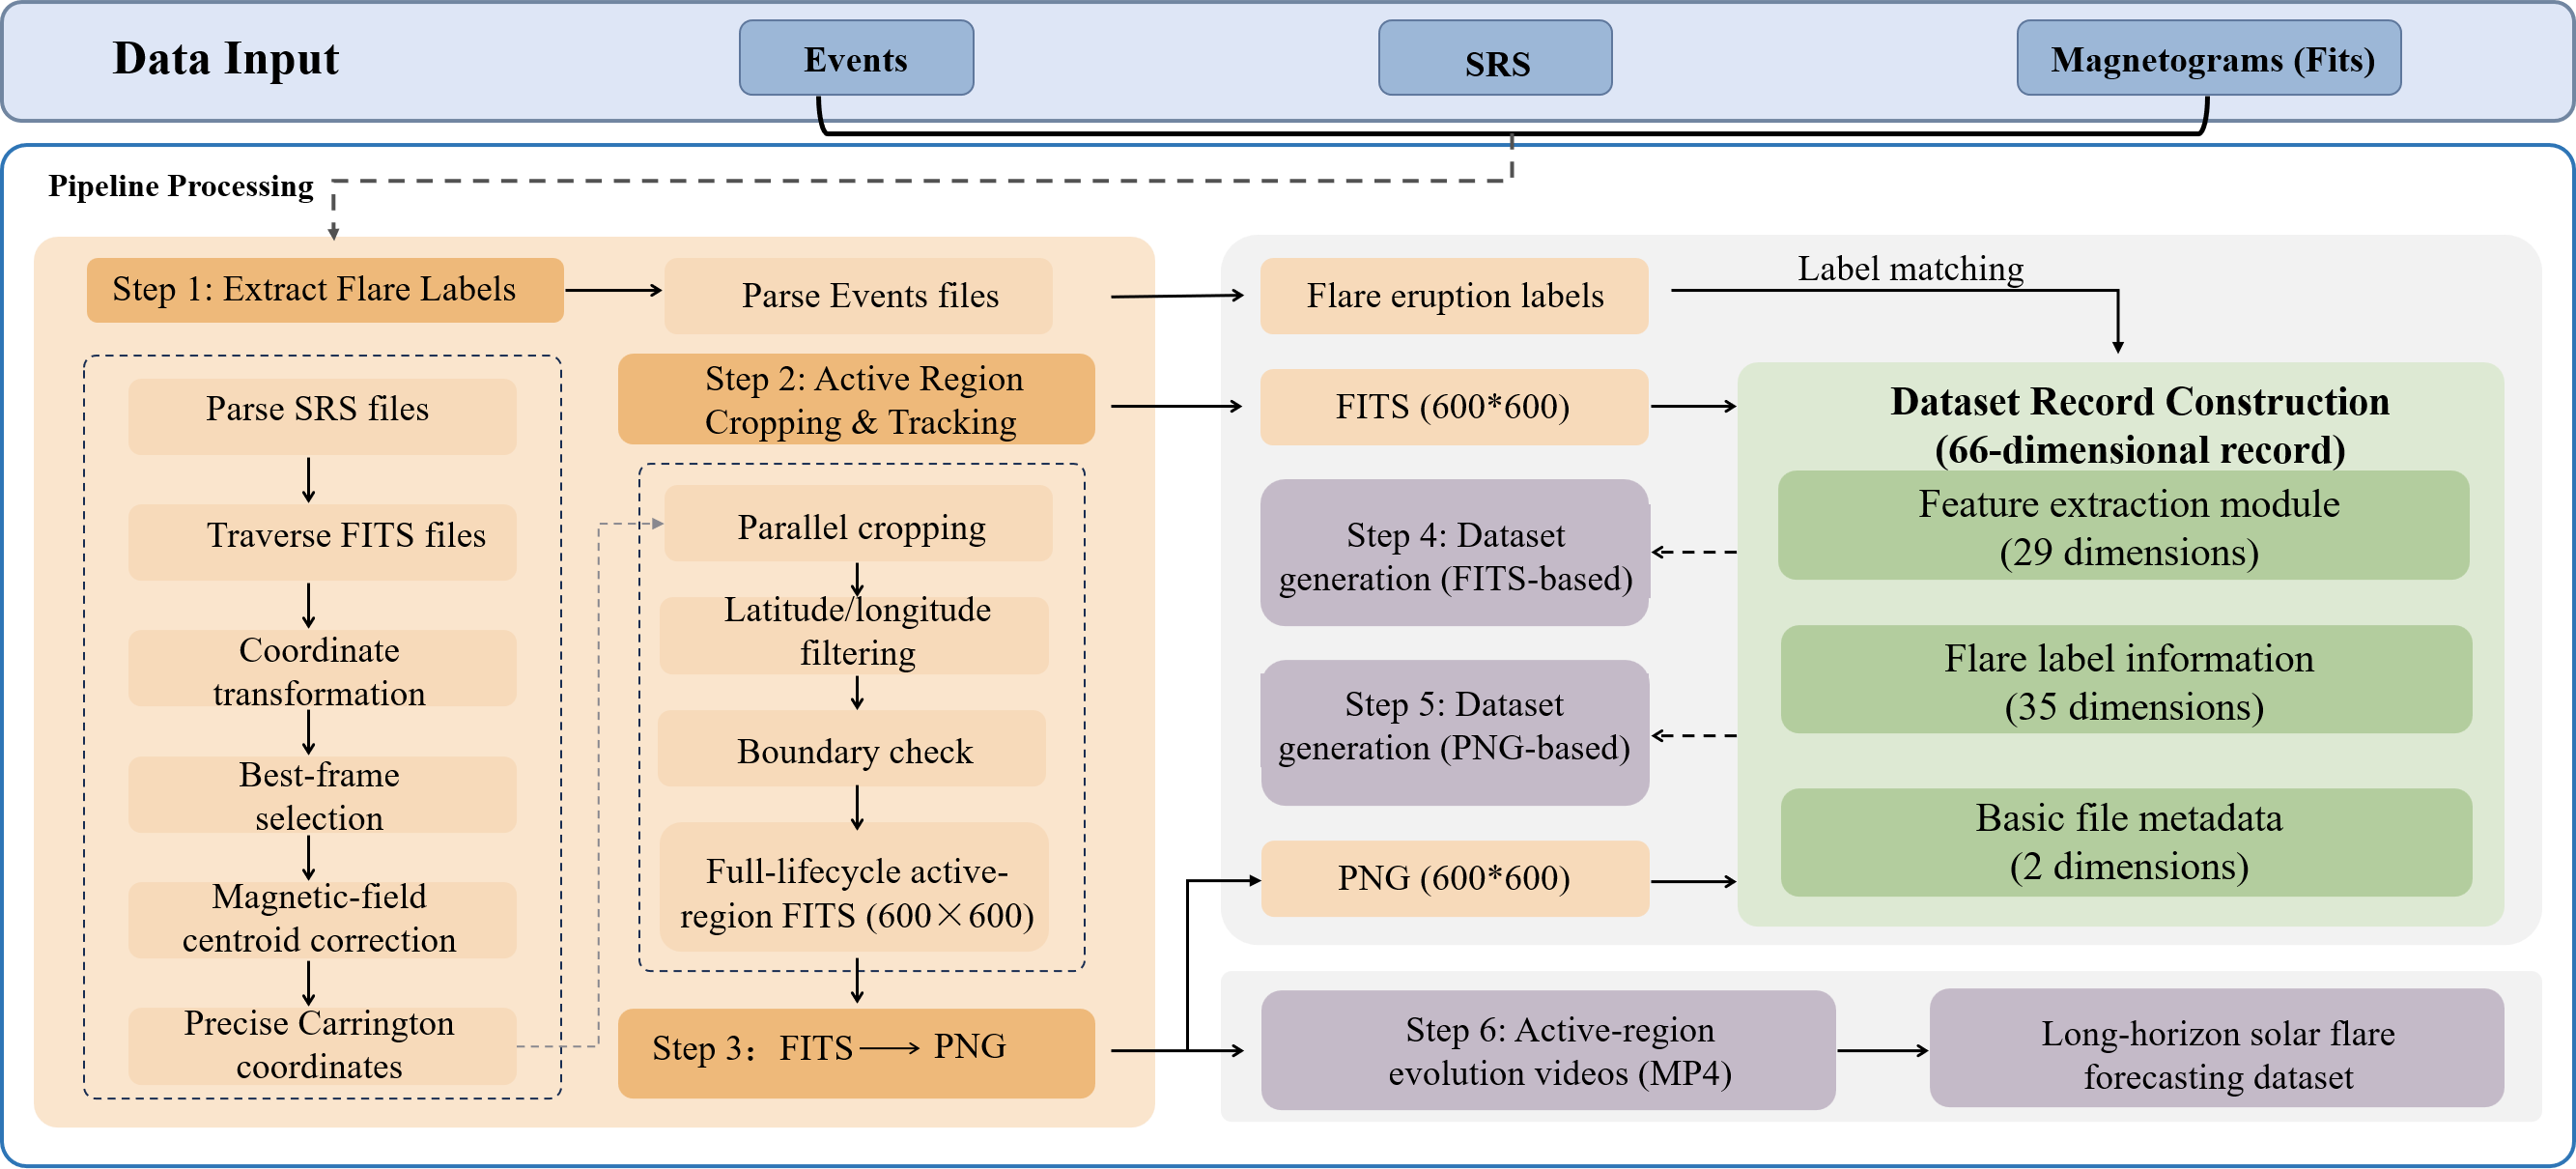
\includegraphics[width=\textwidth]{figures/pipeline.png}
\caption{JW-FD dataset construction workflow. NOAA Events supply flare ground truth; SRS reports and HMI full disk magnetograms define active region crops. Steps~4 and~5 extract the same 29 dimensional feature set and share label matching logic on FITS and PNG branches, respectively.}
\label{fig:pipeline}
\end{figure}

\begin{table}[H]
\caption{Pipeline step inputs and outputs. Here $B_{\mathrm{th}}$ denotes the magnetic saturation threshold (in Gauss) applied when converting FITS magnetograms to 8 bit PNG images; the release includes branches at $B_{\mathrm{th}} \in \{200,400,600,800,1000,2000\}$~G.}
\label{tab:pipeline}
\centering
\scriptsize
\setlength{\tabcolsep}{4pt}
\begin{tabularx}{\textwidth}{@{}c>{\raggedright\arraybackslash}X>{\raggedright\arraybackslash}X>{\raggedright\arraybackslash}X@{}}
\toprule
\textbf{Step} & \textbf{Script} & \textbf{Input} & \textbf{Output} \\
\midrule
1 & \texttt{step1\_extract\_flare\_labels} & NOAA Events \texttt{.txt} (XRA) & \texttt{flare\_labels.csv} \\
2 & \texttt{step2\_crop\_active\_regions} & SRS + HMI FITS (4096$^2$) & \texttt{fits\_600/\{AR\}/} \\
3 & \texttt{step3\_convert\_to\_png} & Step~2 FITS & \texttt{png\_600\_Th\{$B_{\mathrm{th}}$\}/} \\
4 & \texttt{step4\_generate\_dataset\_fits} & FITS + labels & FITS branch CSV \\
5 & \texttt{step5\_generate\_dataset\_png} & PNG + labels & PNG branch CSV \\
6 & \texttt{step6\_make\_movie} & PNG sequences & \texttt{movies/AR\{num\}\_evolution.mp4} \\
\bottomrule
\end{tabularx}
\end{table}

\subsection{Data Sources}

\textbf{SDO/HMI} provides full disk LoS magnetograms at 4096$\times$4096 pixels ($\sim$1.5$''$ per pixel) with a cadence of approximately 12~minutes. \textbf{NOAA/SWPC SRS} reports list daily NOAA AR numbers and heliographic locations~\cite{NOAA2024events}. \textbf{NOAA Events} files record GOES soft X-ray flare begin, maximum, and end times, together with GOES class strings (C, M, or X followed by a numeric subclass).

\subsection{Design Choices}
\label{sec:design}

Four design choices distinguish JW-FD from SHARP based patch datasets and earlier AR image datasets~\cite{Boucheron2023,Bobra2014}.

\textbf{Long temporal coverage.} Fifteen calendar years (2011--2025) span the declining phase of Solar Cycle~24, the 2018--2020 minimum, and the rising phase of Cycle~25. This span supports cycle dependent statistics and supplies enough rare M and X class events for threshold specific studies.

\textbf{Multimodal coregistration.} Every sample is indexed by NOAA AR number and Coordinated Universal Time (UTC) timestamp across FITS magnetograms (Gauss scale physics), PNG frames (vision model input), 29 dimensional magnetic feature vectors, configurable flare labels, and per AR MP4 evolution videos. Users may train end to end vision models on PNG or MP4 inputs, tabular classifiers on extracted features, or MLLMs that fuse imagery with structured metadata~\cite{Shao2025jwflare}.

\textbf{Configurable labels with forecasting semantics.} Binary and class labels are defined for seven forecast horizons ($h \in \{1,3,6,12,24,48,72\}$~hours) and four GOES thresholds ($\tau \in \{\mathrm{C1.0,M1.0,M5.0,X1.0}\}$). Positive labels are assigned only within the half open interval before eruption $[\mathrm{Begin}-h,\,\mathrm{Begin})$, excluding frames after eruption (Figure~\ref{fig:label_timeline}). This definition separates forecasting from nowcasting and matches operational lead time requirements.

\textbf{AR level evaluation split.} Consecutive HMI frames of the same AR exhibit strong temporal autocorrelation, so assigning different timestamps of one AR to both training and test sets constitutes information leakage~\cite{Barnes2016,Leka2019}. JW-FD therefore adopts an 8:1:1 random split at the AR level (Section~\ref{sec:validation}).

Additional practical choices include: (i)~600$\times$600~pixel crops ($\sim$300$''$ field of view); (ii)~NOAA AR centered directory organization rather than HMI Active Region Patch (HARP)/SHARP patch identifiers, matching operational numbering; (iii)~a disk center filter ($|\mathrm{longitude}| \le 60^\circ$) to reduce limb projection effects; and (iv)~dual FITS and PNG CSV branches so that physics faithful (Gauss scale) and vision ready (normalized intensity) feature extraction share identical label logic.

% Figure 2: Pre-eruption label window semantics
\begin{figure}[H]
\centering
\small
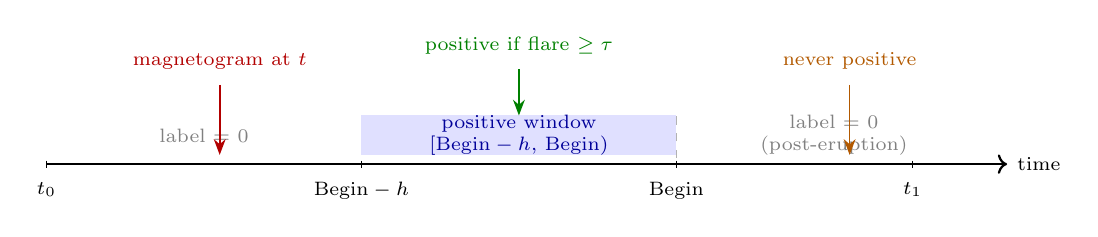
\begin{tikzpicture}[
  x=1.0cm, y=0.65cm,
  lbl/.style={font=\scriptsize},
  arr/.style={-{Stealth[length=2mm]}, semithick}
]
  \draw[thick,->] (0,0) -- (12.2,0) node[right, lbl] {time};

  \foreach \x/\t in {0/{$t_0$}, 4/{$\mathrm{Begin}-h$}, 8/{$\mathrm{Begin}$}, 11/{$t_1$}} {
    \draw (\x,0.07) -- (\x,-0.07);
    \node[lbl, below=3pt] at (\x,0) {\t};
  }

  \draw[dashed, gray!60] (8,0.12) -- (8,1.05);

  \fill[blue!12] (4,0.18) rectangle (8,0.95);
  \node[lbl, blue!60!black, align=center] at (6,0.56)
    {positive window\\$[\mathrm{Begin}-h,\,\mathrm{Begin})$};

  \node[lbl, gray] at (2.0,0.56) {label = 0};
  \node[lbl, gray, align=center] at (10.0,0.56) {label = 0\\{\scriptsize (post-eruption)}};

  \draw[arr, red!70!black] (2.2,1.55) -- (2.2,0.18);
  \node[lbl, red!70!black, above=2pt] at (2.2,1.55) {magnetogram at $t$};

  \draw[arr, green!50!black] (6.0,1.85) -- (6.0,0.95);
  \node[lbl, green!50!black, above=2pt] at (6.0,1.85) {positive if flare $\geq\tau$};

  \draw[arr, orange!70!black] (10.2,1.55) -- (10.2,0.18);
  \node[lbl, orange!70!black, above=2pt] at (10.2,1.55) {never positive};
\end{tikzpicture}
\caption{Strict pre-eruption labeling semantics for horizon~$h$. A magnetogram observed at time~$t$ receives a positive binary label for threshold~$\tau$ only if $t \in [\mathrm{Begin}-h,\,\mathrm{Begin})$ and the matched GOES class meets or exceeds~$\tau$. Observations at or after $\mathrm{Begin}$ (dashed line) are excluded, distinguishing forecasting from nowcasting.}
\label{fig:label_timeline}
\end{figure}


\subsection{Active Region Cropping and Tracking}

Tracking begins from the SRS Stonyhurst location of each NOAA AR at its first available magnetogram time, which is converted to a Carrington anchor. That anchor is then carried across subsequent epochs so that the same heliographic region remains centered as the Sun rotates. Local refinement masks pixels stronger than $100$~G inside an 80 pixel neighborhood of the projected center and updates the center to their mass centroid. From each full disk FITS frame we extract a $600\times600$ crop and discard ARs with $|\mathrm{longitude}| > 60^\circ$.

\subsection{FITS to PNG Conversion}

To obtain vision ready 8 bit inputs, each cropped FITS magnetogram is mirrored left to right into the north up, east left display orientation. Field values are then clipped at a chosen saturation threshold and linearly mapped to the integer range $[0,255]$:
\begin{equation}
B' = \mathrm{clip}(B,\,-B_{\mathrm{th}},\,B_{\mathrm{th}}), \quad
I = \frac{B' - \min(B')}{\max(B') - \min(B')} \times 255,
\label{eq:norm}
\end{equation}
Invalid (NaN) samples are filled prior to clipping. We publish PNG trees for $B_{\mathrm{th}} \in \{200, 400, 600, 800, 1000, 2000\}$~G; Section~\ref{sec:threshold} discusses how this choice affects downstream models.

\subsection{Feature Extraction and Label Matching}

Steps~4 and~5 generate CSV datasets from FITS and PNG inputs. Both branches extract the same 29 feature types and apply the same label matching logic, but the numerical computation differs slightly: FITS features are computed on Gauss scale magnetograms, whereas PNG features are computed on intensity scale images after a 128 level offset. Features follow the methodology of Boucheron et al.~\cite{Boucheron2015}: seven gradient statistics, thirteen neutral line descriptors, five Haar wavelet subband energies, and four magnetic flux integrals.

Each CSV row corresponds to one magnetogram time stamp. We define seven forecast horizons $h \in \{1,3,6,12,24,48,72\}$~hours and four GOES thresholds $\tau \in \{\mathrm{C1.0,M1.0,M5.0,X1.0}\}$. A binary field \texttt{flare\_label\_\{$\tau$\}\_\{$h$hr\}} is set to~1 when at least one flare in the same AR has GOES class $\ge\tau$ and a begin time $\mathrm{Begin}$ lying in the half open window before eruption
\begin{equation}
\mathrm{Begin} - h \;\le\; t \;<\; \mathrm{Begin}
\label{eq:window}
\end{equation}
and is set to~0 otherwise. The companion field \texttt{flare\_class\_\{$h$hr\}} records the maximum GOES class among events that meet the window for horizon~$h$, or \texttt{0} when no such event occurs.

\subsection{Evolution Videos}

For each AR directory, PNG frames are sorted chronologically and encoded as H.264 MP4 at 60~frames per second. Each AR produces one \texttt{AR\{num\}\_evolution.mp4} file in the \texttt{movies/} directory.

\subsection{Quality Control and Expert Verification}
\label{sec:qc}

Automated filters are applied stage by stage. In Step~1, flare records are dropped when the AR identifier is invalid, the peak time is missing, or the GOES class string cannot be parsed. Step~2 removes geometrically invalid crops, including those whose centers leave the usable disk or whose AR longitude exceeds the configured limit. Downstream stages handle I/O failures explicitly: truncated FITS reads are logged in Step~3, while Steps~4--5 skip empty or unreadable files and write per-file errors to the step logs; NaNs encountered in PNG normalization are replaced in place. Consistency of the released split is checked against \texttt{dataset\_split\_log\_PNG\_62\_Th1000.txt} so that row counts agree with the parent tables.

After the automated pass, solar physicists reviewed a random 5\% subset, focusing on crop centering, boundary completeness, and whether M/X class labels align with the intended windows before eruption. Frames compromised by telemetry gaps or rare processing failures were removed or regenerated.

\section{Results}
\label{sec:results}

\subsection{Dataset Records and Statistics}
\label{sec:records}

Processed data follow a consistent directory hierarchy under the release root. Table~\ref{tab:summary} summarizes principal scale metrics; Table~\ref{tab:yearly} reports snapshot counts by calendar year; Table~\ref{tab:modalities} describes each modality; Table~\ref{tab:schema} defines the 66 dimensional CSV record; and Table~\ref{tab:split} documents the evaluation split.

\begin{table}[H]
\caption{JW-FD dataset scale summary (2011--2025 release, PNG branch $B_{\mathrm{th}}=1000$~G).}
\label{tab:summary}
\centering
\small
\begin{tabularx}{\textwidth}{@{}>{\raggedright\arraybackslash}p{4.5cm}X@{}}
\toprule
\textbf{Item} & \textbf{Value} \\
\midrule
Temporal coverage & 2011-01-01 -- 2025-12-31 (15~yr) \\
Active regions & 3{,}064 independent NOAA ARs \\
Magnetogram snapshots & 1{,}991{,}247 \\
Spatial resolution & 600$\times$600~pixels per crop \\
Modalities & FITS, PNG, CSV, MP4 (3{,}064 videos) \\
NOAA flare label records & 12{,}298 (\texttt{flare\_labels.csv}) \\
Standard split & 8:1:1 by AR (train / val / test) \\
Data sources & SDO/HMI LoS; NOAA/SWPC SRS; NOAA Events (XRA) \\
\bottomrule
\end{tabularx}
\end{table}

% Figure 3: Snapshot counts by year (PNG Th1000)
\begin{figure}[H]
\centering
\small
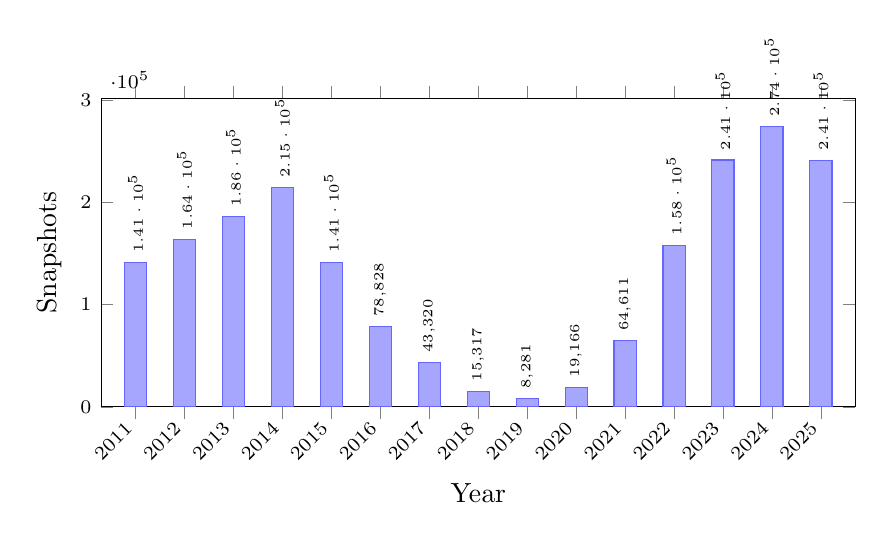
\begin{tikzpicture}
  \begin{axis}[
    ybar,
    bar width=8pt,
    width=0.92\textwidth,
    height=5.5cm,
    ymin=0,
    ylabel={Snapshots},
    xlabel={Year},
    symbolic x coords={2011,2012,2013,2014,2015,2016,2017,2018,2019,2020,2021,2022,2023,2024,2025},
    xtick=data,
    x tick label style={rotate=45, anchor=east, font=\scriptsize},
    y tick label style={font=\scriptsize},
    nodes near coords,
    every node near coord/.append style={font=\tiny, rotate=90, anchor=west},
    enlarge x limits=0.05,
  ]
    \addplot[fill=blue!35, draw=blue!60] coordinates {
      (2011,141005) (2012,164070) (2013,185954) (2014,214503) (2015,141304)
      (2016,78828) (2017,43320) (2018,15317) (2019,8281) (2020,19166)
      (2021,64611) (2022,158002) (2023,241428) (2024,274395) (2025,241063)
    };
  \end{axis}
\end{tikzpicture}
\caption{Number of co-registered magnetogram snapshots per calendar year in the JW-FD release (PNG branch, $B_{\mathrm{th}}=1000$~G). Counts reflect solar-cycle activity: Solar Cycle~24 peak years (2013--2014, 2023--2025) dominate; the 2018--2020 minimum is clearly visible.}
\label{fig:year_chart}
\end{figure}


\begin{table}[H]
\caption{Magnetogram snapshot counts by calendar year (PNG branch, $B_{\mathrm{th}}=1000$~G).}
\label{tab:yearly}
\centering
\small
\begin{tabular}{@{}lr@{\hspace{1.2em}}lr@{\hspace{1.2em}}lr@{}}
\toprule
\textbf{Year} & \textbf{Count} & \textbf{Year} & \textbf{Count} & \textbf{Year} & \textbf{Count} \\
\midrule
2011 & 141{,}005 & 2012 & 164{,}070 & 2013 & 185{,}954 \\
2014 & 214{,}503 & 2015 & 141{,}304 & 2016 & 78{,}828 \\
2017 & 43{,}320 & 2018 & 15{,}317 & 2019 & 8{,}281 \\
2020 & 19{,}166 & 2021 & 64{,}611 & 2022 & 158{,}002 \\
2023 & 241{,}428 & 2024 & 274{,}395 & 2025 & 241{,}063 \\
\midrule
\multicolumn{5}{l}{\textbf{Total (2011--2025): 1{,}991{,}247}} \\
\bottomrule
\end{tabular}
\end{table}

\begin{table}[H]
\caption{JW-FD modalities and file organization.}
\label{tab:modalities}
\centering
\small
\begin{tabularx}{\textwidth}{@{}>{\raggedright\arraybackslash}p{1.5cm}>{\raggedright\arraybackslash}p{1.3cm}X>{\raggedright\arraybackslash}p{3.8cm}@{}}
\toprule
\textbf{Modality} & \textbf{Format} & \textbf{Description} & \textbf{Path pattern} \\
\midrule
FITS & \texttt{.fits} & LoS magnetogram in Gauss; 600$\times$600 crop & \texttt{fits\_600/\{ARnum\}/...} \\
PNG & \texttt{.png} & 8 bit grayscale; saturation $B_{\mathrm{th}}$ in path & \texttt{png\_600\_Th\{B\_th\}/\{ARnum\}/...} \\
CSV & \texttt{.csv} & 66-D record per snapshot; FITS and PNG branches & \texttt{label/\{fits|png\}/Th\{B\_th\}/...} \\
MP4 & \texttt{.mp4} & Per AR evolution video, 60~fps & \texttt{movies/AR\{num\}\_evolution.mp4} \\
Labels & \texttt{.csv} & NOAA XRA flare events & \texttt{flare\_labels.csv} \\
\bottomrule
\end{tabularx}
\end{table}

\begin{table}[H]
\caption{66 dimensional CSV record structure.}
\label{tab:schema}
\centering
\small
\begin{tabularx}{\textwidth}{@{}>{\raggedright\arraybackslash}p{2.8cm}c>{\raggedright\arraybackslash}X@{}}
\toprule
\textbf{Block} & \textbf{Dim.} & \textbf{Content} \\
\midrule
Magnetic features & 29 & Gradient (7), neutral line (13), wavelet (5), flux (4) \\
Binary flare labels & 28 & 7 horizons $\times$ 4 thresholds \\
Class labels & 7 & Strongest GOES class per horizon \\
File metadata & 2 & \texttt{image\_filename}, \texttt{image\_path} \\
\midrule
\textbf{Total} & \textbf{66} & \\
\bottomrule
\end{tabularx}
\end{table}

Example label column names include \texttt{flare\_label\_M1.0\_24hr} (binary) and \texttt{flare\_class\_24hr} (string). The composite key (\texttt{AR\_Number}, UTC timestamp) uniquely identifies each snapshot across modalities.

\begin{table}[H]
\caption{Train/validation/test split (AR level 8:1:1; random seed~62; PNG branch $B_{\mathrm{th}}=1000$~G).}
\label{tab:split}
\centering
\small
\begin{tabular}{@{}lrr@{}}
\toprule
\textbf{Partition} & \textbf{Snapshots} & \textbf{ARs} \\
\midrule
Training & 1{,}592{,}952 & 2{,}450 \\
Validation & 193{,}375 & 307 \\
Test & 204{,}920 & 307 \\
\midrule
\textbf{Total} & \textbf{1{,}991{,}247} & \textbf{3{,}064} \\
\bottomrule
\end{tabular}

\vspace{4pt}
\noindent\footnotesize Sample level GOES class counts (full dataset): X: 15{,}094; M: 129{,}776; C: 422{,}548; no flare (0): 1{,}423{,}829.
\end{table}

\subsection{Magnetic Saturation Threshold Ablation}
\label{sec:threshold}

Converting Gauss scale FITS magnetograms to 8 bit PNG requires a saturation level $B_{\mathrm{th}}$ in Equation~(\ref{eq:norm}). This choice affects visual contrast, feature statistics on PNG derived branches, and model input distributions. JW-FD therefore releases PNG branches at six saturation levels: 200, 400, 600, 800, 1000, and 2000~G.

To provide an initial reference point, we ran a controlled ablation over these thresholds with a Transformer based vision classifier on the PNG branch, using binary flare grade $\geq$C1.0 and the fixed AR level 8:1:1 split (random seed~62). In this internal study, $B_{\mathrm{th}} = 1000$~G yielded the highest skill (true positive rate, TPR~$= 0.6320$; true skill statistic, TSS~$= 0.5225$ for $\geq$C1.0), as reported in Table~\ref{tab:threshold}.

\begin{table}[H]
\caption{Preliminary magnetic saturation threshold ablation (Transformer, $\geq$C1.0, AR level split). Values from internal benchmark; users should re-evaluate for their model and task.}
\label{tab:threshold}
\centering
\small
\begin{tabular}{@{}ccc@{}}
\toprule
\textbf{$B_{\mathrm{th}}$ (G)} & \textbf{TPR} & \textbf{TSS} \\
\midrule
200 & --- & --- \\
400 & --- & --- \\
600 & --- & --- \\
800 & --- & --- \\
\textbf{1000} & \textbf{0.6320} & \textbf{0.5225} \\
2000 & --- & --- \\
\bottomrule
\end{tabular}

\noindent{\footnotesize Complete ablation metrics will be deposited with the dataset release documentation. The 1000~G branch is recommended as a \emph{default starting point} only.}
\end{table}

We emphasize that this threshold selection is a preliminary exploration limited to the Transformer architecture and the $\geq$C1.0 binary task. The optimal saturation may differ for other models (CNN, vision transformer (ViT), MLLM), flare thresholds (M1.0, X1.0), or forecast horizons. Because JW-FD releases PNG branches at all six $B_{\mathrm{th}}$ values, users should treat 1000~G as a recommended starting point rather than a universal optimum and re-ablate when performance is critical.

\section{Discussion}
\label{sec:discussion}

\subsection{Evaluation Protocol and Class Imbalance}
\label{sec:validation}

JW-FD adopts an \textbf{8:1:1 random split at the AR level} with random seed~62: all snapshots of a given AR appear exclusively in the training, validation, or test partition (Table~\ref{tab:split}). This protocol prevents information leakage arising from temporal autocorrelation within ARs~\cite{Barnes2016,Leka2019}. Split CSV files (\texttt{*\_train.csv}, \texttt{*\_val.csv}, \texttt{*\_test.csv}) are distributed under \texttt{label/png/Th\{threshold\}/} and \texttt{label/fits/}.

Positive labels are rare for high thresholds (M5.0, X1.0) and long horizons, producing pronounced class imbalance. Metrics such as the TSS or the Brier score are therefore preferred over raw accuracy~\cite{Bloomfield2012}.

\subsection{Recommended Usage}
\label{sec:usage}

JW-FD is intended for the heliophysics and space weather ML communities. Suggested applications include:

\begin{itemize}
\item \textbf{Vision and video models}: Train CNNs, ViTs, or temporal models on PNG snapshots or MP4 evolution sequences, selecting $B_{\mathrm{th}}$ by ablation (Section~\ref{sec:threshold}).
\item \textbf{Tabular ML}: Apply classical classifiers or gradient boosted trees to the 29 dimensional magnetic feature vectors, comparing FITS derived (Gauss scale) and PNG derived (intensity scale) branches.
\item \textbf{Multimodal and MLLM approaches}: Fuse PNG/MP4 inputs with tabular features and label metadata in a single indexed record~\cite{Shao2025jwflare}.
\item \textbf{Multi horizon benchmarking}: Evaluate models across seven forecast horizons and four GOES thresholds using the precomputed label columns.
\item \textbf{Comparison with prior datasets}: JW-FD extends the temporal span and modality coverage of earlier AR magnetogram datasets~\cite{Boucheron2023}.
\end{itemize}

To reproduce or extend the dataset, clone the open source pipeline at \url{https://github.com/Xiaoxuan-1/JW-FD} and set \texttt{START\_YEAR=2011}, \texttt{END\_YEAR=2025} in \texttt{config.py}. We recommend using the distributed split files so that evaluations remain comparable across publications.

\subsection{Limitations}
\label{sec:limitations}

Current limitations include: (1)~LoS magnetograms only; vector magnetic field products (e.g., SHARP) are not yet integrated~\cite{Bobra2014}; (2)~dependence on NOAA AR numbering and SRS daily positions; (3)~disk center bias induced by the $|\mathrm{longitude}| \le 60^\circ$ filter; and (4)~the 12-minute HMI cadence, which may undersample rapidly evolving configurations before flares.

\section{Conclusions}

JW-FD is a 15 year multimodal solar flare forecasting dataset covering 3{,}064 active regions and 1.99~million coregistered magnetogram snapshots. The release provides FITS, PNG, CSV, and MP4 modalities with 66 dimensional records, configurable labels defined before eruption, and an AR level evaluation split. PNG branches at six magnetic saturation thresholds support input format studies; 1000~G is recommended as a preliminary default, subject to the caveats discussed above. We intend JW-FD to serve as shared infrastructure for classical ML, deep vision, and MLLM based flare forecasting research.

\authorcontributions{Conceptualization, S.M. and J.L.; methodology, S.M.; software, S.M. and L.T.; validation, S.M., H.W. and Y.L.; data curation, S.M.; writing---original draft preparation, S.M.; writing---review and editing, S.M., J.L., H.W., L.T., C.Y., Y.Z. and Y.L.; visualization, S.M.; supervision, H.W.; project administration, S.M. All authors have read and agreed to the published version of the manuscript.}

\funding{This research received no external funding.}

\institutionalreview{Not applicable.}

\informedconsent{Not applicable.}

\dataavailability{The JW-FD dataset described in this paper will be made publicly available upon publication. Processed data are organized under a release root containing \texttt{fits\_600/}, \texttt{png\_600\_Th\{threshold\}/}, \texttt{label/}, \texttt{movies/}, and \texttt{flare\_labels.csv}. A DOI will be assigned upon deposition in a public repository (e.g., Zenodo). The open source dataset construction pipeline is available at \url{https://github.com/Xiaoxuan-1/JW-FD}. Until publication, interested researchers may contact the corresponding author.}

\acknowledgments{Open SDO/HMI magnetograms and NOAA/SWPC flare products made this release possible; we gratefully acknowledge both teams. Support from the National Astronomical Observatories, Chinese Academy of Sciences, is also acknowledged.}

\conflictsofinterest{The authors declare no conflicts of interest.}

\abbreviations{Abbreviations}{
The following abbreviations are used in this manuscript:\\

\noindent
\begin{tabular}{@{}ll}
AR & Active region \\
CNN & Convolutional neural network \\
CSV & Comma separated values \\
FITS & Flexible Image Transport System \\
GOES & Geostationary Operational Environmental Satellite \\
HARP & HMI Active Region Patch \\
HMI & Helioseismic and Magnetic Imager \\
LoS & Line of sight \\
LSTM & Long short term memory \\
ML & Machine learning \\
MLLM & Multimodal large language model \\
MP4 & MPEG-4 video format \\
NOAA & National Oceanic and Atmospheric Administration \\
PNG & Portable Network Graphics \\
SDO & Solar Dynamics Observatory \\
SHARP & Space-weather HMI Active Region Patch \\
SRS & Solar Region Summary \\
SWPC & Space Weather Prediction Center \\
TPR & True positive rate \\
TSS & True skill statistic \\
UTC & Coordinated Universal Time \\
ViT & Vision transformer \\
XRA & X-ray flare event list
\end{tabular}
}

\begin{adjustwidth}{-\extralength}{0cm}
\bibliography{references}
\end{adjustwidth}

\end{document}
